% !TEX root = replicas_draft.tex

\section{Two intervals in the eternal black hole}
\label{sec:TwoIntervals}

We now turn to the information paradox in the eternal black hole \cite{Almheiri:2019yqk}, described in the introduction and pictured in fig.~\ref{fig:eternalBH-lorentzian}. In the late-time regime relevant to the information paradox, the generalized entropy, including the island, is simply twice the answer for a single interval. We would like to understand how this is reproduced from wormholes. This is essentially just putting together the general discussion of section \ref{sec:Action} with the single-interval results of section \ref{sec:SingleInterval}, so we will be brief. We will only discuss the saddles near $n=1$; it would be nice to have a more complete understanding of the finite-$n$ wormholes in this setup.

\subsection{Review of the QES}

We set $\beta = 2\pi$. The points in fig.~\ref{fig:eternalBH-lorentzian} have $(\sigma, t)$ coordinates
\be \la{4pts}
P_1 = (-a, t_a) \ , \quad
P_2 = (b, t_b) \ , \quad
P_3 = (-a, -t_a + i \pi) \ , \quad
P_4 = (b, -t_b + i \pi) \ .
\ee
The radiation region is
\be
R = [P_4, \infty_L) \cup [P_2, \infty_R) \ ,
\ee
and the island is
\be
I = [P_3, P_1] \ .
\ee
The CFT state is pure on the full Cauchy slice, so
\be
S_{\rm CFT}(I \cup R) = S_{\rm CFT}( [P_4, P_3] \cup [P_1, P_2] ) \ .
\ee
This entropy is non-universal; it depends on the CFT. In the theory of $c$ free Dirac fermions \cite{Casini:2005rm}, the entanglement entropy of the region
 \be \la{region}
  [x_1, x_2] \cup [x_3, x_4] ~,
 \ee  with metric $ds^2 = \Omega^{-2} dx d\bar x $, is
\be \la{entrexp}
 S_{\rm fermions} 
= \frac{c}{6}\log \left[ \frac{|x_{21} x_{32}  x_{43}  x_{41} |^2}{
  |x_{31}  x_{42} |^2 \Omega_1\Omega_2\Omega_3\Omega_4} \right] \ .
\ee
where we dropped the UV divergences. 
With our kinematics and conformal factors, this gives
\begin{align}\label{bosonee}
S_{\rm fermions}(I \cup R) 
= \frac{c}{3}\log\left[
\frac{ 2\cosh t_a \cosh t_b \left|\cosh(t_a-t_b) - \cosh(a+b)\right| }{ 
\sinh a \cosh (\frac{a+b - t_a - t_b}{2}) \cosh( \frac{a + b + t_a + t_b}{2}) } 
\right]
\end{align}
In a general CFT, the two-interval entanglement entropy is a function of the conformal cross-ratios $(z,\bar{z})$ which agrees with \eqref{bosonee} in the OPE limits $z \to 0$ and $z \to 1$. For concreteness we will do the calculations for the free fermion, but the regime of interest for the information paradox will turn out to be universal.

The generalized entropy, including the island, is
\be\label{SgenFermion}
S_{\rm gen}(I \cup R) = 2S_0 + \frac{2\phi_r}{\tanh a} +   S_{\rm fermions}(I \cup R) \ ,
\ee
%where $\Delta S_{\rm fermion} = S_{\rm fermion}  + \frac{c}{3}\log \epsilon_{UV}$.
Without an island, the entropy is the CFT entropy on the complement of $R$, the interval $[P_4, P_2]$, which is
\be
S_{\rm gen}^{\rm no~island}= S_{\rm fermions}(R) = 
 \frac{c}{3}\log \left(
{2 \cosh t_b } 
\right)
\ee
At $t=0$, 
\be \la{IslandSgen}
S_{\rm gen}^{\rm island}  = 2 S_0 + \frac{2\phi_r}{\tanh a} + \frac{c}{3}\log \left(
\frac{4 \tanh^2 \frac{a+b}{2} }{  \sinh a}
\right) \ .
\ee
The extremality condition $\p_a S_{\rm gen}^{\rm island} = 0$ at $t_a=t_b = 0$ gives
\be \la{eqnFer}
\frac{6\phi_r}{c} \sinh (a+b) = 2 \sinh^2 a - \sinh a \cosh a \sinh(a+b) \ .
\ee
Whether this has a real-valued solution depends on the parameters $b$ and $\phi_r/c$. For example, if $b=0$, then it has a real solution minimizing $S_{\rm gen}^{\rm island}$ when $\phi_r/c$ is small, but not otherwise. 

At late times, the extremality condition $\p_a S_{\rm gen}^{\rm island} = 0$ always has a real solution. The true entropy, according to the QES prescription, is 
\be
S(R) =
\min\left\{ S_{\rm gen}^{\rm no ~island} \ ,   S_{\rm gen}^{\rm island}   \right\} \ .
\ee
The island always exists and dominates the entropy at late times, because the non-island entropy grows linearly with $t$, see   fig.~\ref{Page}. This solution is in the OPE limit where we can approximate the entanglement entropy by twice the single-interval answer,
\be
S_{\rm matter}(I \cup R) \approx 2 S_{\rm matter}^{\rm   } ([P_1, P_2]) =
 \frac{c}{3}\log \left(
\frac{2|\cosh(a+b) - \cosh(t_a-t_b)|}{
\sinh a} 
\right) \ .
\ee
and the QES condition sets $t_a = t_b$. 

\subsection{Replica wormholes} 


We would like to discuss some aspects of the wormhole solutions that lead to the island prescription. 

For general $n$ these are wormholes which have the topology shown in figures \ref{fig:2wormhole}(b), \ref{fig:manyreplicas}. 
Already from these figures we can derive the  $S_0$-dependent contribution \nref{OrigAct} 
since it involves only the topology of the manifold. The replica wormhole that involves nontrivial connections, 
see figure   
\nref{fig:manyreplicas}, has the topology of a sphere with $n$ holes. This gives a contribution going like 
$Z_n \propto e^{ S_0( 2-n)}$ and a contribution of $2S_0 = (1 - n\partial_n) \log Z_n   |_{n=1}$ \,  for the von Neumann entropy. This is good, since the island contribution 
indeed had such a term \nref{IslandSgen}. 


It is useful to assume replica symmetry and view the Riemann surface as arising from a single disk with 
$n$ copies of the matter theory and with pairs of twist operators that connect all these $n$ copies in a cyclic fashion, see figure \ref{CoverThree}. In order to find the full answer, we need to solve the equations \nref{EOMFin} \nref{PartSing}. The important point is that, at this stage, we have that $n$ appears purely as a parameter and we can analytically continue the equations in $n$. 
  We have not managed to solve the equations for finite $n$. 
But let us discuss some properties we expect. 
In the limit of large $c \beta/\phi_r$, it is likely that solutions exist in Euclidean signature.\footnote{For low values of $c\beta/\phi_r$ we have already seen, in \nref{eqnFer}, that near $n\sim 1$ the solutions can be complex.} 
We can put points 
$P_2$ and $P_4$ at  $v=\pm B e^{ \pm i \varphi }$.   Once this solution is found, we can analytically continue $\varphi \to - i t$ to generate the Lorentzian solution. 
That Lorentzian solution at late times $t$ is expected to exist even for low values of $c \beta/\phi_r$.
In principle, it should be possible, and probably easier,  to analyze directly the late-times Lorentzian equation. 
In fact, 
 we expect that there should be a way to relate the single interval solution to the two interval solution in this regime. The intuitive reason is that at late times the distance between the two horizons is increasing and so the distance between the two cosmic branes is increasing.  We have an external source cosmic brane outside the gravitational region, at the tip of region $R$. 
 The cosmic brane has some tension, as well as a twist operator on it. For the Hawking saddle, the one without the replica wormholes, the twist operators, and the topological line operators\footnote{These topological line operators exchange the $n$ copies in a cyclic way. They are represented by red lines in figure \ref{CoverThree}(b).} that connect them, generate a contribution that grows linearly in time, due to the behavior of 
 Renyi entropies for the matter quantum field theory, as well as the fact that the wormhole length grows with time. 
   At late times the topological line operator can break by pair producing cosmic branes, with their twist operators. The cost of creating a pair of cosmic branes is finite in the gravitational region, because the dilaton is finite. This cost would be infinite in the non-gravitational region. 
  But once the external cosmic brane is screened by the cosmic brane that appeared in the gravity region we expect to have two approximately  independent single interval problems. The reason is that the distance between the left and right sides is growing with time.
  This is somewhat analogous to two point charges that generate a two dimensional electric field. As one separates the charges it might be convenient to create a pair of charges that screens the electric field. For this it is important that the charges one creates have finite mass.
 
 
 In the $n\to 1$ limit we can analyze the solution and we get the generalized entropy. This is not too surprising since the arguments in \cite{Dong:2017xht} say that this should always work. Here the non-trivial input is the ansatz for the configuration of intervals which follows from the structure of the Riemann surfaces. As discussed in section \ref{sec:CosmicStrings}, the effective action reduces to the action of certain cosmic  branes which are manifestly very light in the $n\to 1$ limit. So in this case, the argument of the previous paragraph can be explicitly checked and one indeed obtains that we get the sum over the two single interval problems \cite{Almheiri:2019yqk}. 
  

\subsection{Purity of the total state}


One can take the perspective that our model is defined via a quantum theory living on the flat space region including its boundary endpoints. The global pure state we consider should be a pure state of this region, and a natural question is whether this is captured in the gravity description. Replica wormholes do indeed capture this feature.

The computation of the entropy of this region is given by evaluating the path integral on the manifold shown in figure \ref{FullIntervalSheets}. The branch cuts split the entire flat space region including its boundaries, identifying one half of one sheet with the other half of the next sheet. The most obvious gravitational saddle is the one that connects these consecutive sheets and thereby naturally extending the branch cut through the entire gravity region. A simple rearranging of these sheets shows that this contribution to the Renyi entropy factorizes. This disconnected saddle satisfies $Z_n = Z_1^n$, and evaluating the on shell action on this configuration will give vanishing entropy since
\begin{align}
\Tr \rho^n = {Z_n \over Z_1^n} = 1\,.
\end{align}
This saddle clearly dominates over all other configurations. 

\begin{figure}
\begin{center}
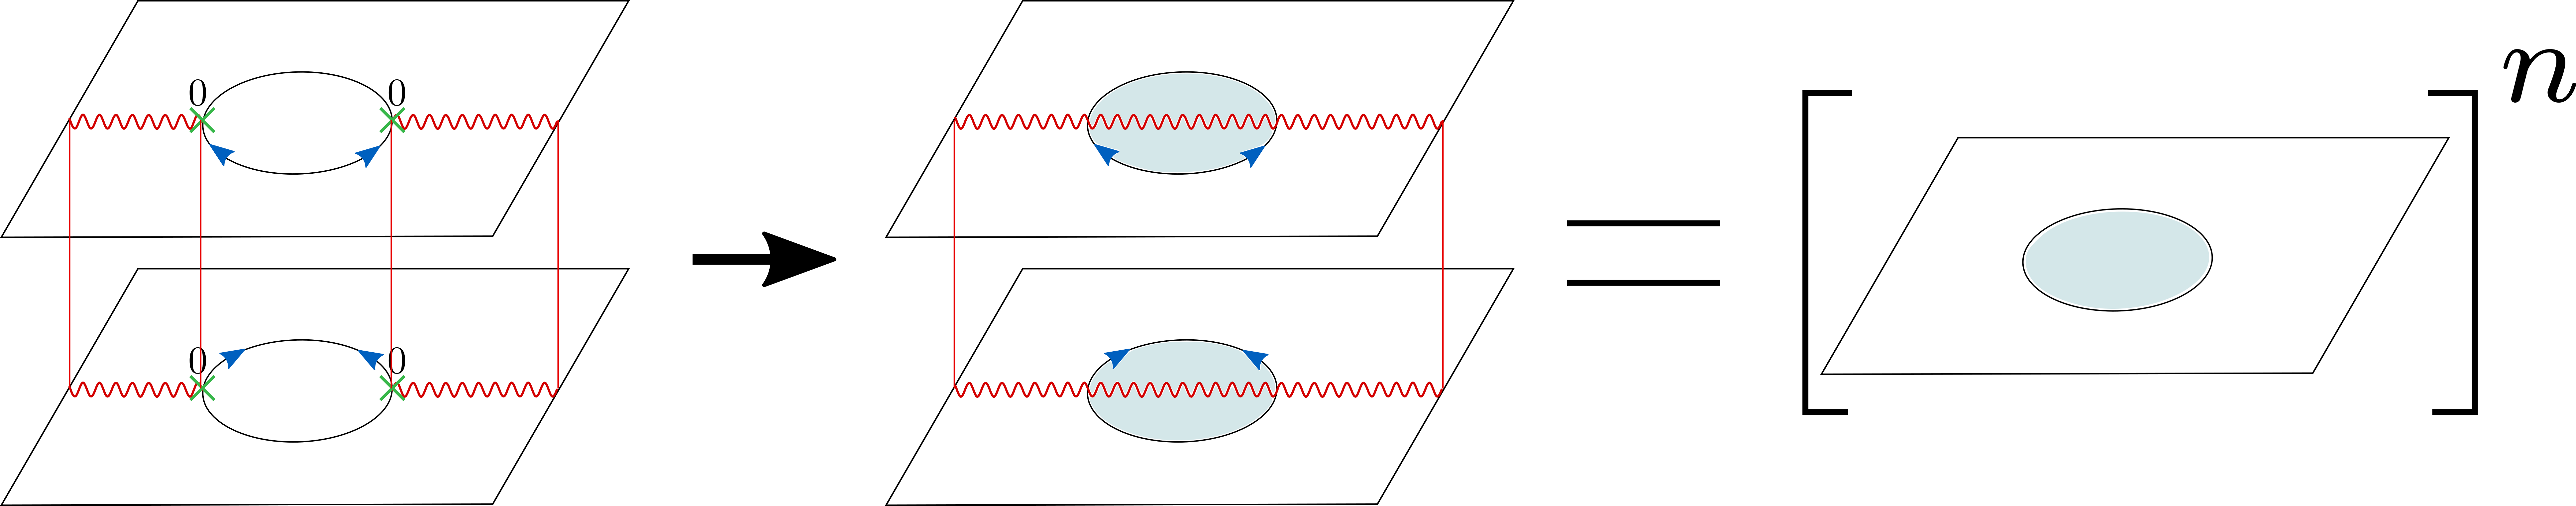
\includegraphics[scale=0.3]{figures/FullIntervalSheets.jpg}
\end{center}
\caption{\small The computation of the entropy of the entire flat space regions including the boundary points. The dominant gravitational saddle connects consecutive sheets. This factorizes into $n$ separate sheets and produces a vanishing entropy consistent with the purity of the flat space region union the endpoints. The blue arrows indicate how the unit circle is identified across the cut.
\label{FullIntervalSheets}}
\end{figure}

Since the different sheets are not coupled at all in the flat space region, it's plausible that this disconnected saddle is the only saddle that exists. Other off-shell contributions can indeed exist, but we speculate they should give a vanishing contribution in a model with a definite Hamiltonian with no averaging.





